\subsection{Modelli Compartimentali}
% scrivere stato dell'arte simile a chapter 2 pg.33 pdf book (download)
In epidemiologia i modelli compartimentali sono una tecnica di modellezione 
generica che si predispone molto bene allo studio complessivo del comportamento
di una malattia infettiva \cite{wiki:Compartmental_models_in_epidemiology}. 
Questa tecnica di modellazione si applica anche ad altre branche della 
scienza, una tra tutte la finanza.

Questa tecnica di modellazione matematica basa il proprio funzionamento 
sull'assunzione che, data una popolazione di individui, questi vengano 
etichettati in maniera differente, in base allo stato di progressione 
della malattia che hanno, o non hanno, contratto. Così facendo si vanno a 
definire dei compartimenti ben separati che possono interagire tra loro, ma 
che rimangono chiaramente distinti l'uni dagli altri.

\subsubsection*{Equazioni Ordinarie Differenziali}
Un equazione ordinaria differenziale (ODE) è un equazione che coinvolge alcune derivate
ordinarie di una funzione. \cite{wiki:Equazione_differenziale_ordinaria} Generalmente data una 
derivata di una funzione si vuole studiare la funzione di partenza e per fare questo bisogna trovare 
l'antiderivata (o integrale) della funzione in esame. 

$$\frac{dx}{dt}(t) = cos(t) \rightarrow x(t) = sin(t) + C$$

Generalmente però risolvere una ODE è più complicato di risolvere un semplice integrale, e pur sapendo 
che il principio alla base rimane la risoluzione di un integrale, la parte difficile è quella di determinare
quale tipo di integrazione abbiamo bisogno per ricavare la nostra soluzione.

Fintanto che le equazioni associate a $\frac{dx}{dt}$ dipendono esclusivamente dalla variabile $t$ e non 
dalla funzione $x(t)$ allora la loro risoluzione risulta molto più facile di quanto non sembri. Tuttavia 
nel caso in cui si avesse una funzione che dipende da $x(t)$ questo ragionamento si fa più complicato.
Nel caso in cui $\frac{dx}{dt}$ dipende da $x(t)$ non è possibile applicare una semplice integrazione e 
successivamente il teorema fondamenteale del calcolo \cite{wiki:Fundamental_theorem_of_calculus}, ma anzi 
necessitiamo di effettuare alcune manipolazioni, in particolare quelle che prendono il nome di \emph{chain rules}
o \emph{u-substitution}.

\subsubsection{Il modello Kermack-McKendrick}
Secondo la definizione precedente possiamo separare la popolazione soggetta di studio 
in categorie, o compartimenti, e assumere una relazione temporale che descriva il passaggio 
di individui da un compartimento all'altro. Malattie che garantiscono un immunità avranno 
una struttura compartimentale differenti da malattie che non la garantiscono.

Il modello che tutt'ora viene usato come riferimento e come base per 
lo studio e modellazione è il così detto modello 
\textbf{Susceptible, Infectious, Recovered} (SIR)

\begin{figure}[h]
    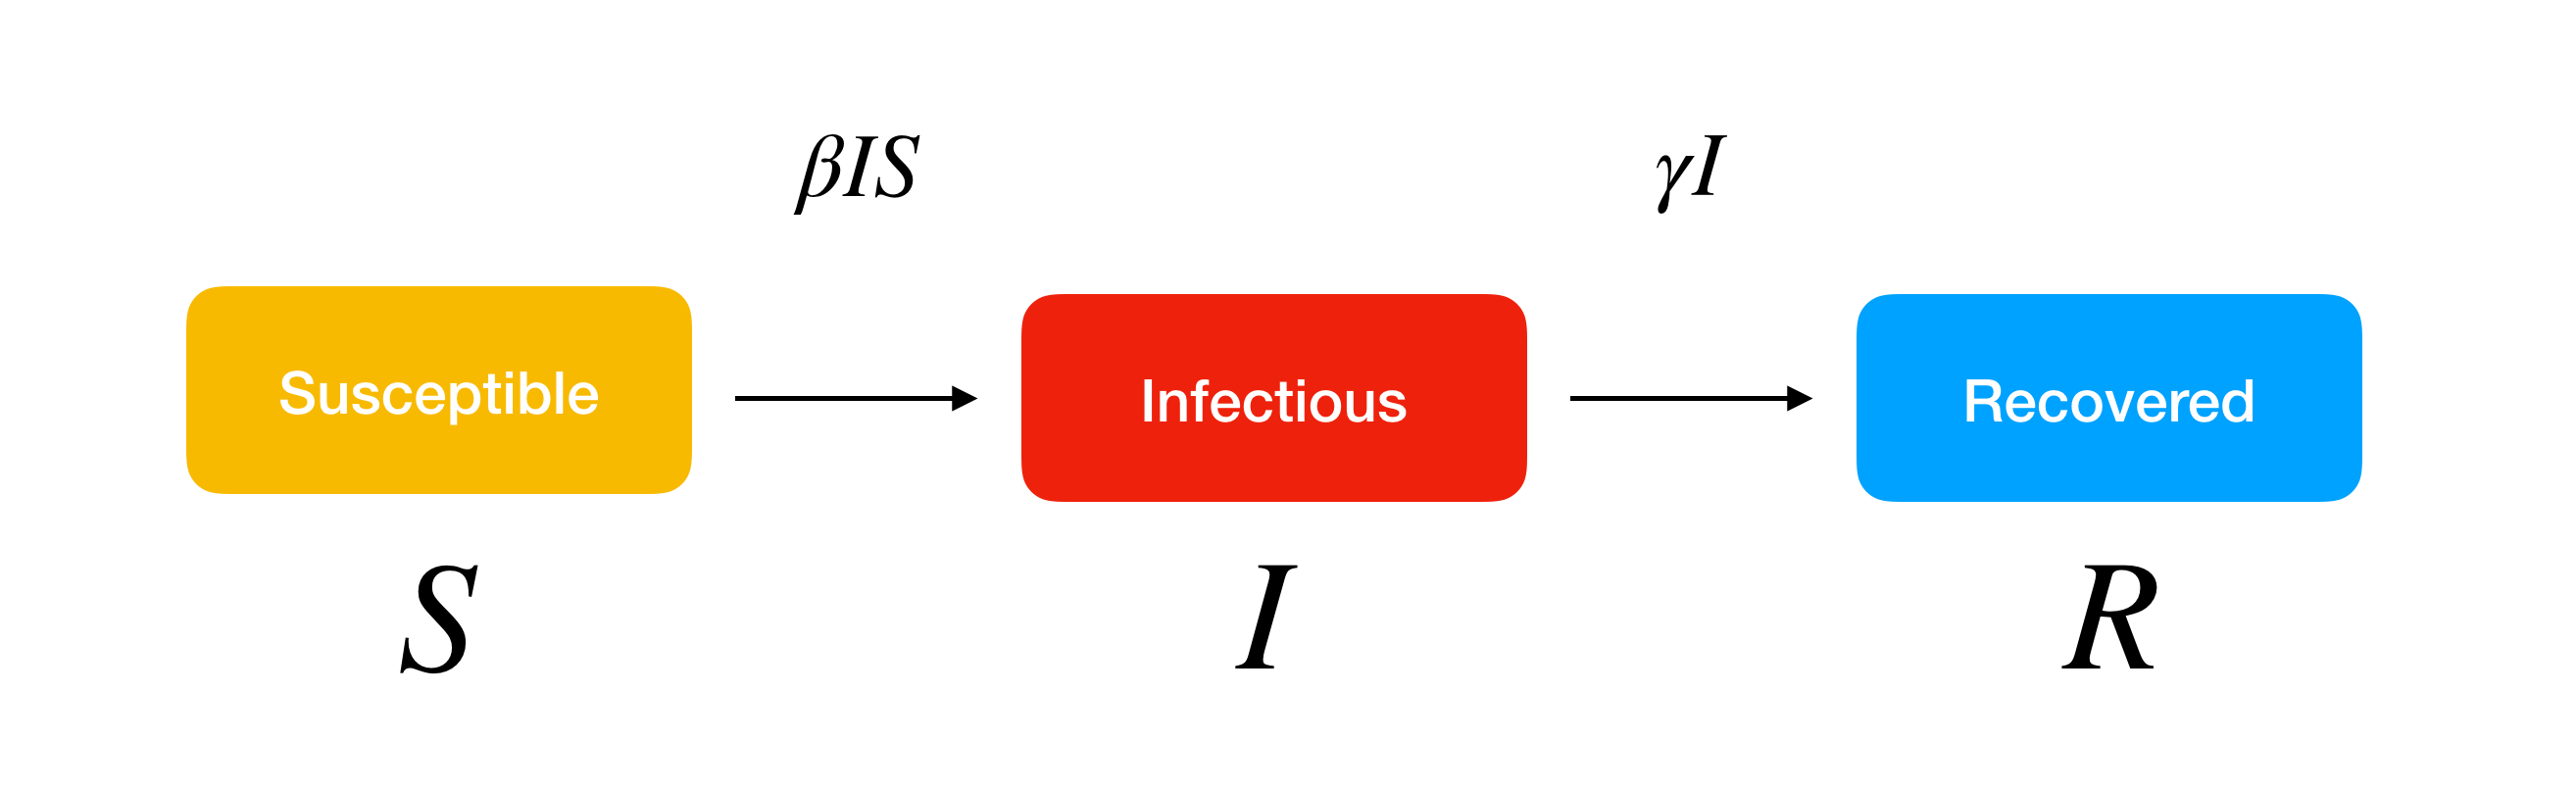
\includegraphics[width=\linewidth]{img/sir.png}
    \caption{Esempio della struttura del modello SIR} 
    \label{fig:SIR_Structure}
\end{figure}

Questo modello è stato ideato all'inizio del 20esimo secolo, 
più precisamente nel 1927, da Kermack e McKendrick. Come introdotto questo modello
si basa sull'assunzione che all'interno di una popolazione durante 
il decorso di una malattia vi possano esistere solamente tre stadi in cui 
un individuo può essere inserito: 

\begin{itemize}
    \item Susceptible: Questo stadio rappresenta lo stato iniziale per la maggior parte
    degli individui all'interno di una popolazione. Rappresenta il numero di 
    persone che possono contrarre la malattia.
    \item Infectious: Questo stadio rappresenta tutti quegli individui che dallo 
    stato di Susceptible, dopo essere venuti in contatto con un individui infetto, 
    diventano a loro volta individui infetti.
    \item Recovered: Questo stadio rappresenta una duplice categoria, quella degli
    individui che alla fine del docorso della malattia sopravvivono ad essa, e 
    quelli che invece muoiono a causa di questa. Generalemente questo stato viene
    anche definito come Removed.
\end{itemize}

Da questa semplice idea poi si è andato a sviluppare un modello
matematico per descrivere come queste 3 categorie separate ma 
che si influenzano vicendevolmente, cambiano nel corso del tempo.
La variabile indipendente del modello è il tempo, indicato come $t$ e il 
tasso di trasferimento tra compartimenti, il quale è espresso matematicamente come 
derivate rispetto al tempo e alla dimensione del compartimento, e come risultato questo 
modello è stato inizialmente formulato tramite l'utilizzo delle equazioni differenziali
\cite{Brauer2008}. 

Durante la formulazione del modello in termini di derivate della dimensione di ogni compartimento
si assume che il numero di individui di ogni compartimento sia rappresentabile come una funzione 
differenziabile nel tempo. Questa assunzione può essere una ragionevole approssimazione nel caso 
in cui vi siano molti individui per compartimento, altrimenti potrebbe risentire di essere sospetta
in caso contrario. Nel caso in cui si utilizzino le equazioni ordinarie differenziali come modello 
si assume che il comportamento della popolazione sia determinato completamente da una relazione deterministica. 
Questa assunzione può essere una ragionevole approssimazione, tuttavia esistono approcci di tipo 
\emph{stocastico} che aggirano questo tipo di assunzione introducendo concetti probabilistici per
la modellazione del modello.

Il modello in figura \ref{fig:SIR_Structure} è un caso speciale del modello proposto da Kermack e McKendrick 
nel loro articolo del 1927, ma è divenuto il modello base per la strutturazione di questo tipo di modelli.
Questa tipologia di modello descrive il seguente sistema di equazioni ordinarie differenziali:

\[
    \left\{
    \begin{array}{ll}
        \frac{dS}{dt} = -\beta \cdot S \cdot I\\
        \frac{dI}{dt} = \beta \cdot S \cdot I - \gamma \cdot I\\
        \frac{dR}{dt} = \gamma \cdot I\\
    \end{array}
    \right.
\]

Questo sistema modella le seguenti assunzioni: 
\begin{itemize}
    \item In media un individuo della popolazione effettua sufficienti contatti con altri individui tale per cui 
    è possibile far evolvere l'infezione con la seguente relazione $\beta \cdot N$ con $N$ numero di individui totali. 
    \item Gli infetti abbandonano il compartimento che determina gli infetti con un tasso pari a $\gamma \cdot I$.
    \item Non esistono entrate o uscite di individui dalla popolazione totale eccezione fatta per possibili uscite tramite morte
    data dalla malattia stessa.
\end{itemize}

Data la descrizione sopra fatta, in accordo con il primo punto, la probabilità di un contatto casuale da un individuo 
infetto con un individuo suscettibile, a cui è possibile trasmettere l'infezione, è di $\frac{S}{N}$, sove il numero di nuovi 
infetti è dato da $(\beta \cdot N) \cdot (\frac{S}{N}) \cdot I = \beta \cdot S \cdot I$. Questo approccio è criticabile in quanto 
si può argomentare come il tasso di contatti dovrebbe essere governato dal numero di infetti e non dei suscettibili, andando 
così a descrivere la seguente formula $(\beta \cdot N) \cdot (\frac{I}{N}) \cdot S = \beta \cdot S \cdot I$. In entrambi i casi 
si ottiene lo stesso tasso di infezione; tuttavia possono esistere approcci dove una scelta sia più adatta dell'altra.

La seconda assunzione non ha una chiara controparte con il mondo epidemiologico. Consideriamo l'insieme dei membri che sono stati infettati 
in un dato periodo di tempo e consideriamo $u(s)$ come il numero di questi che sono ancora infettivi dopo $s$ unità di tempo. Se definiamo 
$\alpha$ come la frazione di infetti che abbandona la classe di appartenenza in un determinato periodo di tempo, otteniamo la seguente formula
$ù = - \alpha u$, la cui soluzione è $u(s) = u(0) e^{-\alpha s}$. Con questo la frazione di infetti che rimangono infettivi dopo un periodo 
$s$ è $e^{-\alpha s}$, per cui il periodo di infettività viene approssimato come una \emph{distribuzione esponenziale} con media 
$\int_{0}^{\infty} e^{-\alpha s} \,ds = \frac{1}{\alpha}$.

Questa assunzione, per cui il tasso di contatto è proporzionale alla dimensione della popolazione $N$ con una costante di 
proporzionalità $\beta$  e una distribuzione esponenziale del tasso di ripresa, è generalmente troppo semplicistica. Tuttavia pur essendo 
un modello che descrive un andamento estremamente semplicistico e irrealistico, è stato osservato come modelli molto più complessi e realistici 
hanno dimostrato comportamenti estremamente simili a questo, facendo si che questo modello, seppur semplice, sia un buon modello che approssima bene 
la realtà.

Il problema definito precedentemente non è possibile da risolvere analiticamente, però da ciò è possibile imparare il comportamento generale del sistema.
Questo approccio permette di inserire un numero variabile di infetti all'interno di una popolazione per studiare se e come 
un'epidemia si propaghi. La quantità $\beta \cdot \frac{S(0)}{\alpha}$ è indicata come una soglia generalmente conosciuta 
come \emph{basic reproduction number} e viene indicato come $R_0$, il quale determina se può o meno avvenire un'epidemia. 
Se $R_0 < 1$ allora l'infezione andrà a morire prima di diventare una epidemia, mentre se fosse $R_0 > 1$ vi sarà 
un outbreak epidemico.

L'indice $R_0$ definisce il numero di infezioni secondarie causate da un singolo individuo durante il proprio periodo infettivo 
all'interno di una popolazione pienamente suscettibile di dimensione $K \approx S(0)$ durante l'intero decorso dell'infezione. In 
questa situazioneun individuo infetto effettua $\beta \cdot K$ contatti per unità di tempo, ognuno di essi con un individuo suscettibile 
che produce nuove infezioni durante un periodo medio infettivo di $\frac{1}{\alpha}$; con questo si può ottenere che il valore di $R_0$ è 
$\beta \cdot \frac{K}{\alpha}$. Generalmente è difficile stimare il rateo di contatto $\beta$ in una popolazione in quanto questo dipende fortemente 
dalla tipologia di malattia studiata ma anche dal comportamento sociale degli individui. Tuttavia esistono molteplici approssimazioni 
che permettono di modellare l'andamento di una malattia infettiva in presenza di pochi dati. 

Il numero di infetti è stato osservato crescere esponenzialmente e questo può essere approssimato dalla seguente formula $ì = (\beta \cdot K - \alpha) \cdot I$
e l'iniziale crescita è definibile come $r = \beta \cdot K - \alpha = \alpha \cdot (R_0 - 1)$. Il valore di $r$ può essere stimato sperimentalmente 
all'inizio di una pandemia. Successivamente, data la possibilità di misurare sia $K$ che $\alpha$, $\beta$ può essere calcolato come 
$\beta = \frac{r + \alpha}{K}$, tuttavia questo approccio è sensibile alla presenza di incompletezza dei dati e alla segnalazione parziale dei casi effettivi, andando 
ad avere una rappresentazione non accurata. Questa sensibilità nell'accuratezza è ulteriormente accentuata quando si studia l'outbreak di una malattia 
precedentemente sconosciuta o in cui i primi casi sono facilmente proni a diagnosi errate.   

\subsubsection{Derivazione modello SIR: modello SEIR}
In molteplici malattie infettive esiste un periodo definito di \emph{esposizione} \cite{wiki:Incubation_period} in cui un individuo una volta infetto non 
è immediatamente infettivo per cui vi è un ritardo nella trasmissione effettiva della malattia. Questo periodo è irrilevante quando è estremamente breve. 
Tuttavia un periodo di esposizione lungo può portare a differenze significative nel modello. Generalmenmte per modellare questa variante è sufficiente 
inserire un nuovo compartimento \textbf{E} il quale va a modificare il sistema di equazioni differenziali nel seguente modo:

\[
    \left\{
    \begin{array}{ll}
        \frac{dS}{dt} = - \beta(N) \cdot S \cdot I\\
        \frac{dE}{dt} = \beta(N) \cdot S \cdot I - \kappa \cdot E\\
        \frac{dI}{dt} = \kappa \cdot E - \gamma \cdot I\\
        \frac{dR}{dt} = \gamma \cdot I\\
    \end{array}
    \right.
\]

Questo modello permette di integrare l'evenienza di casi \emph{asintomatici} i quali sono infettivi e non totalmente 
associabili al compartimento \textbf{E}.

\begin{minipage}{\linewidth}
    \centering
    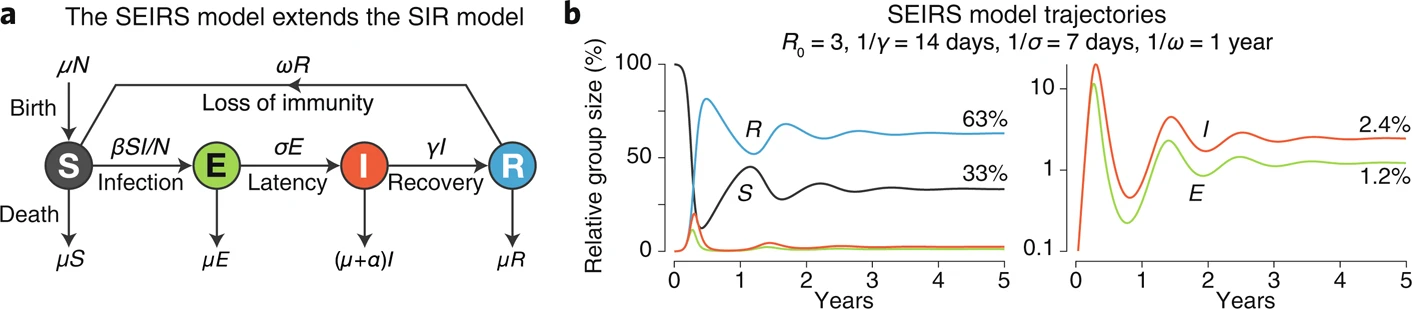
\includegraphics[width=\textwidth]{img/41592_2020_856_Fig1_HTML.png}
    \captionof{figure}{Esempio di modello SEIRS \cite{Bjornstad2020}}
    \label{fig:SEIRS_model}
\end{minipage}

\subsubsection{Modello SIR stocastico}
Una delle assunzioni del modello presentato precedentemente, ovvero della tipologia \textbf{deterministica} è quella per cui la dimensione 
dei compartimenti è abbastanza grande da permettere di avere un mix omogeneo di membri al suo interno. Questa assunzione è sufficientemente
ragionevole quando un'epidemia è già avviata, ma all'inizio la situazione può risultare estremamente differente. All'inizio di una 
epidemia la maggior parte della popolazione ricade all'interno della categoria suscettibile, ovvero che non è stata (ancora) infettata, e il numero associato 
agli individui infetti è relativamente piccolo. Il rateo di trasmissione della malattia dipende fortemente dal pattern dei contatti tra individui e servirebbe utilizzare 
una descrizione di questo pattern. Poichè il numero di infetti è piccolo una descrizione del modello che utilizza una assunzione di \emph{mass action} dovrebbe essere 
sostituito da un modello che incorpora degli effetti stocastici.

\begin{minipage}{\linewidth}
    \centering
    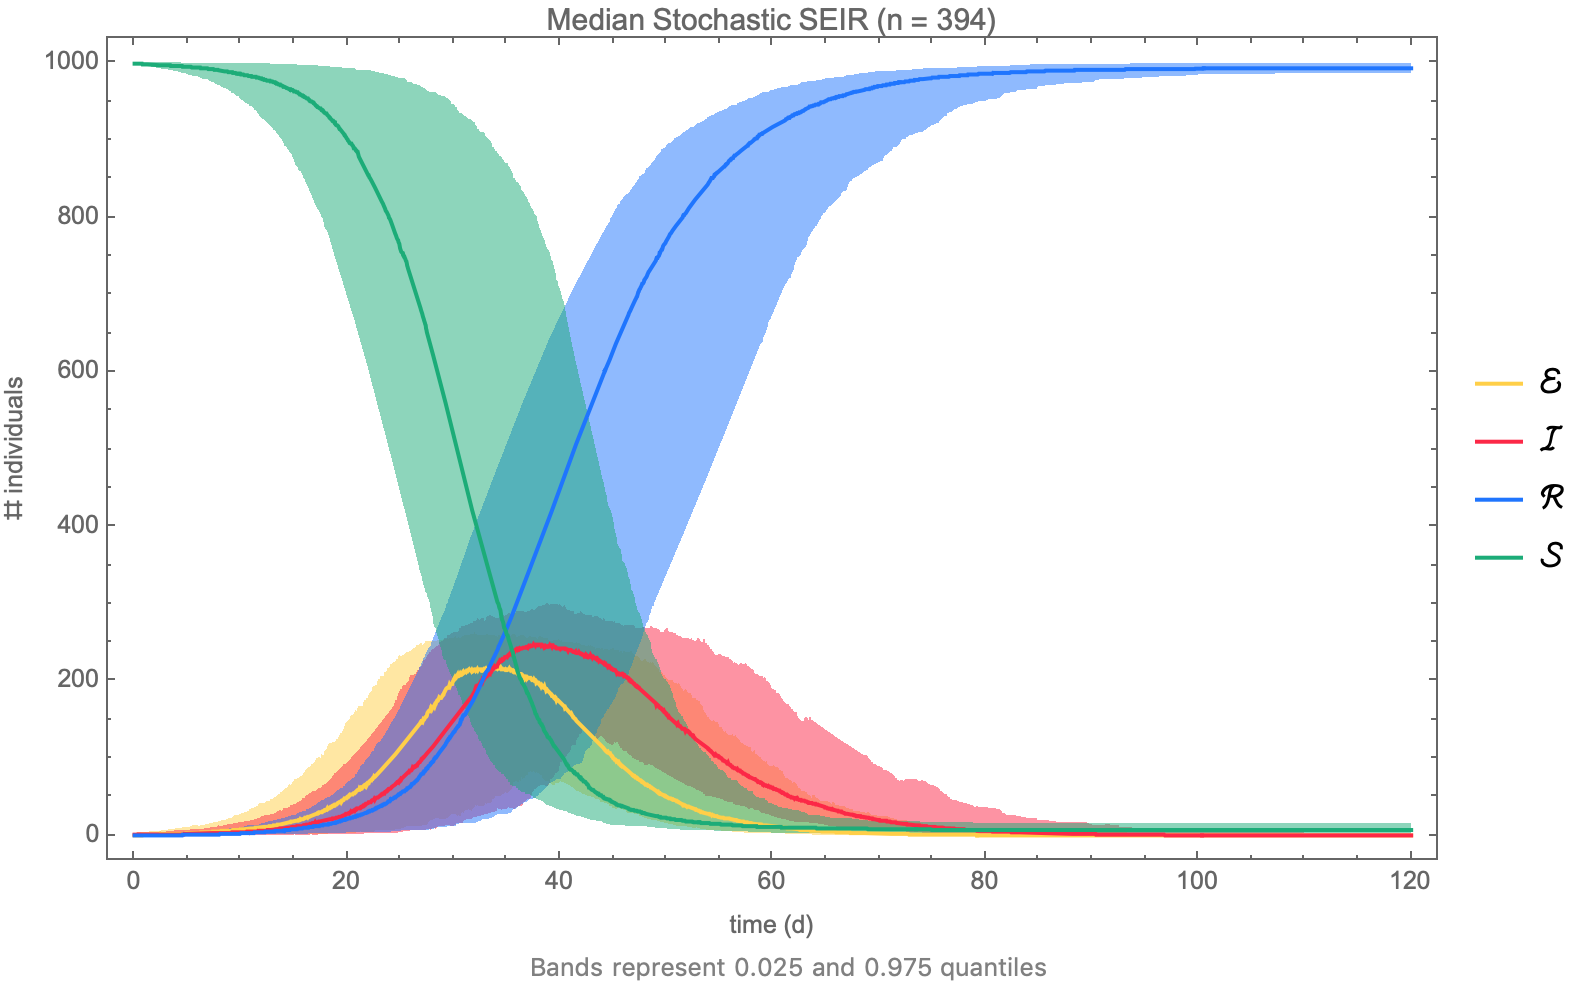
\includegraphics[width=\textwidth]{img/stochastic_SEIR.png}
    \captionof{figure}{Esempio di modello SEIR stocastico}
    \label{fig:stochastic_SEIR_model}
\end{minipage}

Esistono differenti approcci che permettono di descrivere questo comportamento stocastico, il primo e 
sicuramente più intuitivo è quello di descrivere un modello stocastico dell'epidemia. Altrimenti è possibile 
utilizzare un modello stocastico della pandemia per una malattia che può essere comunicata da applicare 
fintanto che il numero di infetti rimane relativamente piccolo, andando a distinguere due differenti categorie:
un \emph{minor disease outbreak} confinato negli stadi iniziali della pandemia e un 
\emph{major disease outbreak} che occorre nel caso in cui il numero di infetti inizia a crescere esponenzialmente.

Una volta che la pandemia è iniziata, è possibile passare ad un modello di tipo deterministico, in questo caso si 
parla di \textbf{network models}.